\documentclass{article}
\usepackage[english]{babel}
\usepackage[round,authoryear]{natbib}
\usepackage{graphicx}
\usepackage{amsmath}
\usepackage[most]{tcolorbox}
\usepackage{hyperref}
\bibliographystyle{abbrvnat}

\title{\textbf{MOCCA} \\[0.25cm]
\large a Multi-sourced Ocean Carbonate Chemistry Analysis \\[1cm]
\textit{or} \\[0.25cm]
\textit{a story about getting the right answer for the wrong reason}}
% maybe also \title{Uncertainties from deep learning in climate science}
% maybe also robustness
% maybe also: Traceability
% Or; epistemic implications of deep learning in cliamte science
% https://www.frontiersin.org/articles/10.3389/frai.2023.974295/full
% https://www.nature.com/articles/s42256-022-00592-3
% https://christophm.github.io/interpretable-ml-book/neural-networks.html
% https://ieeexplore.ieee.org/document/9521221
% https://towardsdatascience.com/dense-or-convolutional-part-2-interpretability-c310a9fd99a5 (only image classification)
% https://en.m.wikipedia.org/wiki/Universal_approximation_theorem
%https://www.scribd.com/document/468040826/Approximation-with-Artificial-Neural-Network-MSc-Thesis-2001-pdf
%https://deeplearningdiary.com/2023/11/26/universal-approximation-theorem-the-infinitely-squiggly-function/
%https://medium.com/analytics-vidhya/you-dont-understand-neural-networks-until-you-understand-the-universal-approximation-theorem-85b3e7677126
%https://ai.stackexchange.com/questions/17670/how-can-supervised-learning-be-viewed-as-a-conditional-probability-of-the-labels
%https://towardsdatascience.com/understanding-objective-functions-in-neural-networks-d217cb068138

% alternatives
% \title{When are machine learning based predictions in climate science accurate?}
% \title{Interpretability of neural-network-based results in climate science?}
% \title{What can be learned from machine learning models in climate science?}
\author{Friedrich Burger}
\date{\today}

\begin{document}
	
	\maketitle
	
	\vspace{10cm}
	Jupyter notebooks with the analyses as well as model weights can be found in the repository \url{https://github.com/friedrichs-repo/MOCCA/}.
	
	
	\newpage
	
	\tableofcontents
	\section{Introduction}
	Deep learning has been heavily used in climate science in recent years \citep{reichstein2019}, with applications ranging from forecasting, statistical down-scaling, pattern identification, process parameterization, emulation of physical models, to data interpolation. The success of deep learning in such data-driven applications is based on the versatility of neural networks~\cite{goodfellow2016}. In theory, these can be used to learn any functional relationship between predictors and variables of interest, as reflected by the universal approximation theorem~\cite{hornik1989}.
	
	A particularly important application of deep learning is the interpolation of sparse ship-based measurements of the fugacity of carbon dioxide (fCO$_2$) in the surface ocean. A globally consistent and complete field of fCO$_2$ is necessary to estimate the air-sea CO$_2$ flux and thus necessary to estimate the fraction of anthropogenic carbon emissions that is taken up by the ocean. The global carbon budget \citep{friedlingstein2023}, an annual assessment of global carbon emissions and sinks, currently estimates the oceanic sink from seven observation-based products. While based on very similar underlying fCO2 data and similar mostly satellite-based predictors, these seven products follow different approaches for interpolating the sparse fCO$_2$ data. 
	
	Four of these products are based on feed-forward neural networks: The CMEMS-LSCE-FFNNv2 \citep{chau2022} utilizes a 100-member neural network ensemble,  bootstrapping from the months before and after a fCO$_2$ measurements and leaving the months with fCO$_2$ measurements for independent evaluation. The MPI-SOMFFN \citep{landschuetzer2016} builds on a two step procedure, where first different clusters of similar ocean conditions are determined using a self-organizing map approach and then neural networks are trained to predict fCO$_2$ in each cluster separately. Similarly, OS-ETHZ-GRaCER \citep{gregor2021} provides an ensemble of varying cluster assignments with neural-network-based fCO$_2$ regression in each cluster. NIES-ML3 \citep{zeng2022} is based on three model estimates, from a random forest, a gradient boost machine, and a feed-forward neural network. The remaining three observation-based products build on multiple linear regressions for A$_\text{T}$ and C$_\text{T}$ \citep[fundamental variables to calculate fCO$_2$ and other carbonate system variables; JMA-MLR;][]{iida2021}, extreme gradient boosting to predict the missfit between global ocean biogeochemical models and fCO$_2$ measurements \citep[LDEO-HPD;][]{gloege2022}, and a autoregressive multiple linear regression approach \citep[Jena-MLS;][]{roedenbeck2022}.
	
	The largest uncertainty in these spatially and temporally interpolated fCO$_2$ fields roots in the sparsity and uneven distribution of the underlying fCO$_2$ measurements that are collected in the Surface Ocean CO$_2$ Atlas~\citep{bakker2016}. In particular, measurements are sparse in high-latitude regions and particularly in the Southern Ocean. One approach to soften this issue is applying neural-network based regression seprately in clusters with similar ocean-biogeochemical conditions \citep{landschuetzer2016,gregor2021}, grouping data-sparse regions with others with similar conditions. The approach taken here, instead, attempts to tackle these limitations by not only using fCO$_2$ measurements for training, but also pH measurements from biogeochemical Argo floats~\citep{johnson2017}, which provide critical additional data in the Southern Ocean, and other biogeochemical data as provided by the Global Ocean Data Analysis Project~\citep[GLODAPv2;][]{olsen2016}. Furthermore, the neural network in MOCCA is pretrained on CMIP6 Earth system models to foster inference of surface fCO$_2$ in sparsely sampled ocean regions with the prior knowledge about functional relationships from Earth system models. The use of multiple sources of data is enabled by a flexible model structure that allows to train on multiple target variables. Similarly to \cite{iida2021}, this flexible approach also aims at providing coherent estimates for all variables of the oceanic carbonate system. However, in the current version, the learning from multiple sources fails, with reductions in loss for the data from the Surface Ocean CO$_2$ Atlas, for example, coming at a prive of increased loss in the other fields.
	
	\section{Overall model architecture}
	\begin{figure}
		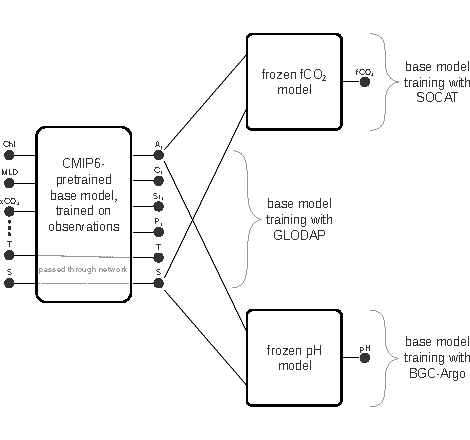
\includegraphics[width=0.85\textwidth]{./figures/model_architecture_scheme.pdf}
		\caption{Scheme displaying the overall model architecture of MOCCA.}
		\label{fig:fco2_model}
	\end{figure}
	MOCCA is based on a three-step procedure~(Figure~\ref{fig:fco2_model}). In a first step, surrogate neural network models are trained to fit the functional relationship between a set of variables needed to solve the oceanic carbonate system (\textit{carbonate chemistry drivers}) and two specific carbonate chemistry variables, pH and fugacity of CO$_2$ (Section~\ref{sect:surrgate_models}). The functional relationship is learned from the numerical carbonate chemistry package \textit{mocsy 2.0} \citep{orr2015}. This step is performed first to identify appropriate hyper parameters and training procedure in a situation where near-perfect learning is possible.
	
	In a second step, a neural network is trained on model output from CMIP6 Earth system models to learn the statistical relationships between a set of predictors and the carbonate chemistry drivers. This model will serve as a prior estimate to improve inference for fCO$_2$ and pH in undersampled regions where only few fCO$_2$ and pH measurements are available.
	
	In a third step, the CMIP6-pretrained model from the previous step is trained with observational data for fCO$_2$ from the Surface Ocean CO$_2$ Atlas (SOCAT), carbonate chemistry drivers from GLODAP, and pH from BGC-Argo floats. To do so, the loss is either directly calculated from the output of the base model (GLODAP), or the fCO$_2$ or pH models are appended to the base model (for SOCAT and BGC-Argo respectively). In the latter case, the layers of the fCO$_2$ or pH models are frozen to prevent further parameter updates.
	
	\section{Surrogate models for mocsy fCO2 and pH} \label{sect:surrgate_models}
	\begin{tcolorbox}[colback=gray!5!white, colframe=black!75!white, 
		fonttitle=\bfseries, title=Jupyter Notebooks, 
		rounded corners, width=\textwidth]
		train\_fco2\_model.ipynb \\
		train\_ph\_model.ipynb
	\end{tcolorbox}
	In a first step, surrogate multi-layer perceptron models were trained to replace numerical solution of the oceanic carbonate system. To do so, samples for total alkalinity (A$_\textup{T}$), dissolved inorganic carbon (C$_\textup{T}$), temperature (T),  salinity (S), total silicate (Si$_\textup{T}$), and total phosphate (P$_\textup{T}$) were randomly generated from uniform distributions (Table~\ref{tab:gen_data}). \\
	The training data size was set to 5 000 000 samples and the validation data size was set to 1 000 000 samples. Mocsy 2.0 (Orr et al., 2015a) was then used to calculate fCO$_2$ and pH for these samples. After normalizing per feature with the means and standard deviations given in Table~\ref{tab:gen_data}, multilayer perceptron models with three identical hidden layers were trained with mocsy fCO$_2$ and pH as labels. \\
	For fCO$_2$, model complexity was iteratively increased until a desired maximum deviation of less than 1\,$\mu$atm was reached (the measurement uncertainty for pCO$_2$ as reported by Orr et al, 2015b)\footnote{For reference, fCO$_2$ across the generated samples varies between 0.001\,$\mu$atm and 5108\,$\mu$atm.}. During training, learning rate was decreased from 10$^{-3}$ to 10$^{-5}$ following an exponential learning rate schedule over 10 000 epochs. The decay in learning rate was chosen to shift from an initial identification of an optimal region in the parameter space to finding an optimal set of parameters for which the mean squared error over the training and validation sets converges to a similar and low value. \\
	Hidden layer size was increased from an initial 64 hidden layer units (8833 trainable parameters), 80 units (13601 parameters), 96 units (19393 parameters), 128 units (34049 parameters), to 160 units (52801 parameters). The largest model\footnote{To give some context about the model complexity: The number of paramters of this model is comparable to that of a Taylor expansion of a function with six arguments to 15th order. Assuming an efficient use of the MLP parameters, a good fit to the numerical solution from mocsy is thus expected.} hit a maximum deviation of 1.08\,$\mu$atm over the validation set (Figure~\ref{fig:fco2_model}).
	The same model architecture was then also used to train the pH model, %albeit with longer training time (14 000 epochs instead of 10 000 for the fCO$_2$ model, extendind the last training step with a learning rate of 10$^{-5}$ to enable convergence on both the training and validation sets), 
	resulting in a maximum deviation over the validation set of 0.0044. \\
	With root mean squared errors (RMSE) of 0.026\,$\mu$atm (fCO$_2$ model) and 0.00008 (pH model), these surrogate models provide a precision that is comparable to numerical carbonate chemistry packages: Orr et al., 2015b report a desired numerical uncertainty of 0.1\,$\mu$atm and 0.0003, respectively. \\
	The accurracy of the fCO$_2$ and pH neural network models is similar for the six million random samples for A$_\text{T}$, C$_\text{T}$, T, S, Si$_\text{T}$, and P$_\text{T}$ from the CMIP6 models (section~\ref{sect:cmip6-pretraining}). Specifically, RMSE is 0.029\,$\mu$atm and 0.00006, respectively, and the maximum deviations are 0.24\,$\mu$atm and 0.0006, respectively.     
	
	\begin{table}
		\centering
		\bgroup
		\def\arraystretch{1.5}
		\begin{tabular}{c|c|c}
			& minimum & maximum \\
			\hline 
			A$_\textup{T}$ & 1000\,$\mu$mol\,kg$^{-1}$ & 3000\,$\mu$mol\,kg$^{-1}$ \\
			\hline
			C$_\textup{T}$ & 1000\,$\mu$mol\,kg$^{-1}$ & A$_\textup{T}$ \\
			\hline
			T & -2\,°C & 35\,°C \\
			\hline
			S & 10\,PSU & 50\,PSU \\
			\hline
			Si$_\textup{T}$ & 0\,$\mu$mol\,kg$^{-1}$ & 134\,$\mu$mol\,kg$^{-1}$ \\
			\hline
			P$_\textup{T}$ & 0\,$\mu$mol\,kg$^{-1}$ & 4\,$\mu$mol\,kg$^{-1}$ \\
			
		\end{tabular}
		\egroup
		\caption{Minima and maxima of the uniform distributions used to generate samples for the fCO$_2$ and pH surrogate models. The range for A$_\textup{T}$ was chosen such that it easily encompasses open ocean variations in A$_\textup{T}$. That for C$_\textup{T}$ is limited to values lower A$_\textup{T}$ since larger C$_\textup{T}$ do not occur in the ocean. The ranges for T and S are chosen according to Lueker et al., 2000, whose parameterizations for K$_1$ and K$_2$ are used in mocsy. Finally, the maximum values for Si$_\textup{T}$ and P$_\textup{T}$ were chosen to be the global maxima found in the monthly climatologies for Si$_\textup{T}$ and P$_\textup{T}$ from World Ocean Atlas 2023. These uniform distributions have means $(max + min) / 2$ and standard deviations $(max - min) / \sqrt{12}$, expcept for C$_\textup{T}$ where mean and standard deviation are given by $min + (max - min) / 4$ and $(max - min) \cdot \sqrt{7 / 144}$, respectively. These means and standard deviations are used for feature normalization.}
		\label{tab:gen_data}
	\end{table}
	\begin{figure}
		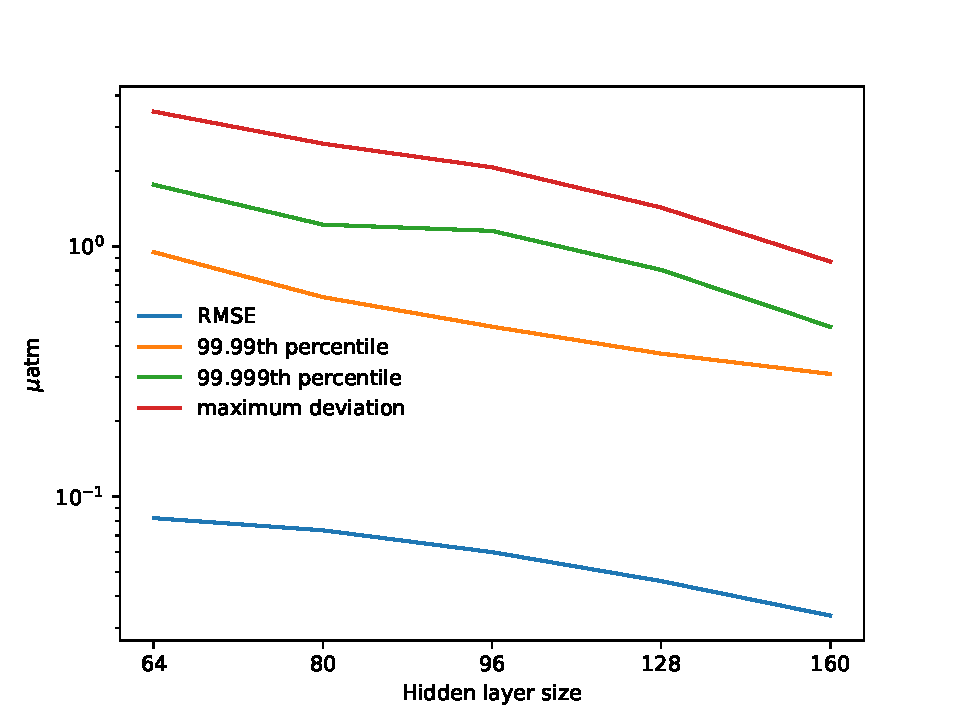
\includegraphics[width=0.85\textwidth]{./figures/fco2_model_error_vs_hidden_layer_size.pdf}
		\caption{The evolution of root mean squared error (RMSE), the 99.99th and 99.999th percentiles of deviation and the maximum deviation between the surrogate model and mocsy fCO$_2$ over the validation data set with 1000 000 randomly generated samples.}
		\label{fig:fco2_model}
	\end{figure}
	\section{CMIP6-pretrained base model} \label{sect:cmip6-pretraining}
	\begin{tcolorbox}[colback=gray!5!white, colframe=black!75!white, 
		fonttitle=\bfseries, title=Jupyter Notebooks, 
		rounded corners, width=\textwidth]
		CMIP6\_data\_preparation.ipynb \\
		train\_CMIP6\_base\_model.ipynb \\
		\textbf{under ./single\_CMIP6\_model\_experiments:} \\
		CMIP6\_data\_preparation\_1model.ipynb \\
		train\_CMIP6\_base\_model\_1model.ipynb \\
		train\_CMIP6\_base\_model\_1model\_with\_cld\_pr.ipynb \\
		train\_CMIP6\_base\_model\_1model\_large\_model.ipynb
	\end{tcolorbox}
%	\begin{itemize}
%		\item say how well the model learns on the 3-CMIP6 model ensemble
%		\item in particular how well it learns just to rescale T and S to the normalization used for the frozen fCO2 and pH models
%		\item Also test how well CMIP6-pretrained model learns on just one climate model (e.g., UKESM) to say how much of the error in A$_\textup{T}$, C$_\textup{T}$, Si$_\textup{T}$ and P$_\textup{T}$ is due to variations in the statistical relationships between predictors and these concentrations between the models
%		\item In final model, test whether excluding pr hurts. Also test for gaussianity and log-transform if that makes variable more gaussian (e.g., check whether skewness and courtosis are smaller after transform (should be zero for a gaussian distribution)), should be relevant for MLD, chl, ice, and pr.
%	\end{itemize}
	As a first step, we pre-train a neural network on the statistical relationships between predictor variables and sea surface A$_\textup{T}$, C$_\textup{T}$, Si$_\textup{T}$, and P$_\textup{T}$. The predictor variables chosen here are sea surface temperature (SST), sea surface salinity (SSS), mixed layer depth (MLD), sea surface height (SSH), chlorophyll-a concentration (chl), sea ice concentration (ice), 10\,m easterly wind (u), 10\,m northerly wind (v),
	% precipitation (pr), cloud cover (cld),
	dry volume molar ratio of CO$_2$ in the atmosphere (CO$_2$), sinus and cosinus of the month of year ($\sin(m / 12 \cdot 2\pi)$ and $cos(m / 12 \cdot 2\pi)$), as well as latitude and longitude encoded using spherical coordinates following \cite{gade2010}. The representations for month of year and location are used to avoid discontinuities in the months between December and January and in longitude at the dateline ($\pm180$\,°E).
	
	The neural network is trained on 6 million samples (5 million for training and 1 million for validation) that were evenly drawn from three CMIP6 Earth system models: the UKESM1-0-LL, the MPI-ESM1-2-LR, and the CMCC-ESM2. Despite a high-resolution version of the MPI model, these were the only ones to provide all predictors on monthly-mean resolution. Data from multiple Earth system models were used to ensure that the model learns general relationships that are not specific to a certain Earth system model with respective biases. The model data is taken from the period 1993-2022 (\textit{historical} simulation until 2014, followed by \textit{SSP2-4.5}). The predictors MLD and chl were log-transformed prior to training to foster learning. The log transformation was applied only where the resulting distribution was more Gaussian (where the test statistic of a Kolmogorov-Smirnov test, i.e. the maximum difference between the empirical distribution function of the data and the distribution function of a standard normal distribution, was smaller after transformation). 
	%SST ans SSS were added to the list of labels for training, since these variables are required as predictors for the downstream fCO$_2$ and pH surrogate models (Figure~\ref{fig:fco2_model}).
	Finally the predictors for the CMIP6 pre-trained base model are nromalized to zero mean and unit variance and the 4 labels are normalized as specified in Table~\ref{tab:gen_data} (to match the normalization used for the fCO$_2$ and pH surrogate models).
	
	For the training, the same architecture that was already used to train the surrogate models (despite not applying a final ELU non-linearity on the output layer, such that the last hidden layer is linearly projected) is used, again with 10\,000 epochs and a batch size of 1000. Root mean squared errors of 6.1\,$\mu$mol\,kg$^{-1}$ (A$_\textup{T}$), 6.3\,$\mu$mol\,kg$^{-1}$ (C$_\textup{T}$), 0.8\,$\mu$mol\,kg$^{-1}$ (Si$_\textup{T}$), and 0.03\,$\mu$mol\,kg$^{-1}$ (P$_\textup{T}$) are obtained (on the validation set and after backtransforming to unnormalized labels). As such, RMSEs are more than a magnitude lower than the standard deviations of A$_\textup{T}$, C$_\textup{T}$, Si$_\textup{T}$, and P$_\textup{T}$ in the CMIP6 model data samples, given by 111.7, 99.1, 26.3, and 0.5\,$\mu$mol\,kg$^{-1}$, respectively\footnote{RMSE equals the standard deviation for a model that always predicts the mean of a variable. Hence, a lower RMSE implies skill in predicting spatial and temporal variations in the variable.}. Likely due to the large size of the training data set relative to the model complexity, overfitting appears not to be a problem. The validation loss continuously decreases, ending up 11\,\% larger than the training loss\footnote{Technically speaking, the training data loss is calculated for all batches in an epoch separately and then averaged. It is thus calculated slightly different than the validation loss.}. %The small error for SST and SSS (max. devation of 0.5°C and 0.4\,PSU across the validation set, respectively) is expected since the neural network only has to learn the normalization for these variables, that are predictors at the same time (Figure~\ref{fig:fco2_model}).
	
	A part of this error can be explained by the fact that the neural network mapping is necessarily imperfect since the three models imply different statistical relationships between predictors and labels. Creating 6 million samples only from the UKESM1-0-LL model, the root mean squared errors become significantly smaller, now being 4.0\,$\mu$mol\,kg$^{-1}$ for A$_\textup{T}$, 4.2\,$\mu$mol\,kg$^{-1}$ for C$_\textup{T}$, 0.5\,$\mu$mol\,kg$^{-1}$ for Si$_\textup{T}$, and 0.02\,$\mu$mol\,kg$^{-1}$ for P$_\textup{T}$. The remaining errors should be mainly due to insufficient information in the predictor variables to fully explain the variations in the four concentrations. Adding further predictors may enhance the skill of a model. However, an experiment with total cloud cover and precipitaion as additional atmospheric predictors resulted only in marginal improvements of errors. In another sensitivity test, the training using UKESM1-0-LL model data was also repeated using a much wider model architecture (256 units per hidden layer, 150\,\% increase in number of parameters). In the first half of the training, validation loss steadily declines, becoming 24\,\% smaller than the validation loss for the default model architecture with 160 units per hidden layer. This highlights a potential for increasing model performance with a larger neural network to a certain extent. In the second half of the training, however, overfitting results in a steady increase in validation loss. As such, a fully-connected neural network of this size requires either more training data to converge without overfitting or some regularization technique. Given that there is an order of magnitude less data availble from observations, the smaller network architecture appears to be a good choice for the next step, where the model is fine-tuned with observational data following a transfer learning protocol. 
	
	\section{SOCAT-, GLODAP-, and BGC-Argo-based model tuning}
	\begin{tcolorbox}[colback=gray!5!white, colframe=black!75!white, 
	fonttitle=\bfseries, title=Jupyter Notebooks, 
	rounded corners, width=\textwidth]
	gridding\_the\_GLODAP\_data.ipynb \\
	gridding\_the\_bgc-argo\_data.ipynb \\
	train\_base\_model\_on\_observations.ipynb
	\end{tcolorbox}
	In this step, the CMIP6-pretrained base model shall be trained on observational data. The data products used for each predictor are listed in Table\,\ref{tab:pred_data} and those used for the label data are listed in Table\,\ref{tab:label_data}. These data are generally on much higher-resolution than the regular 1°-latitude $\times$ 1°-longitude grid used here. As such the data for SST, SSS, MLD, chl, ice, SSH, u, and v were first binned to this coarser reslution. For CO$_2$ a global and annual-average representative value was used. The Surface Ocean CO$_2$ Atlas (SOCAT) provides average fCO$_2$ measurements on the desired 1°$\times$1° grid. The data from GLODAP and BGC-Argo, however is only available as individual un-gridded measurements. These data were gridded here in the jupyter notebooks listed above. From GLODAP, two different types of gridded data were derived; one with all four concentrations (A$_\text{T}$, C$_\text{T}$, Si$_\text{T}$, and P$_\text{T}$) available, and one only with A$_\text{T}$ and C$_\text{T}$ (the more important quantities) available. As a result, four data categories are used here for training and validation: SOCAT, BGC-Argo, GLODAP-4, and GLODAP-2. Removing grid values where not all predicors provide data, these data categories encompass 324296, 9449, 10629, and 3959 gridded values, respectively. 
	
	The 14 predictors (incl. representations of month of year and geographical location as outlined in the last section) were then normalized with the means and standard deviations from the CMIP6 samples. This was done to improve 'out-of-the-box' CMIP6-pretrained model performance on the observational data. Following the scheme in Fig.\,\ref{fig:fco2_model}, a modular MLP was then defined, with the base model with pretrained weights and biases from the CMIP6 data training, the frozen surrogate fCO2 model mapping the output from the base model to fCO$_2$ if a respective flag is provided in the MLP model call, and the frozen surrogate pH model to map the base model output to pH given the respective flag is provided in the model call.
	
	As a first experiment, the model was used to predict fCO$_2$, pH, A$_\text{T}$, C$_\text{T}$, Si$_\text{T}$, and P$_\text{T}$ over the validation sets of the respective data categories SOCAT, BGC-Argo, GLODAP-4, and GLODAP-2. In this zero-shot inference scenario, the model archieved the correct order of magnitude. However, RMSEs of 49.5$\mu$atm, 0.038, 126.6$\mu$mol\,kg$^{-1}$, 114.5$\mu$mol\,kg$^{-1}$,  15.0$\mu$mol\,kg$^{-1}$, and 0.25$\mu$mol\,kg$^{-1}$, respectively, are similar to the sample standard deviations, highlighting limited predictive power.   
	
	In a next step, the base-model should be finetuned on observational data. This approach is motivated by the relatively low amount of observational data compared to model complexity and by the biased distribution of obesrvational data, while climate model data is available everywhere in the world ocean such that a model pretrained on climate model data may be less spatially biased. The idea was to roughly follow the protocoll by \cite{geron2019hands}, who proposes to first retrain the final layer of the base model (a linear projection layer in this case), and then to subsequently unfreeze layers from the output side and fine-tune them with a small learning rate, until model performance on the validation data does not improve anymore. 
	
	When alternatingly training on all four data categories, however, I faced several difficulties. First, the loss on the different data categories is on different orders of magnitude, such that the training will prioritize reducing the loss in one variable over reducing the loss in another variable - with, for example, pH varying much less then fCO2, resulting in much smaller MSEs for pH than for fCO2 and less training success for pH. This problem can be, in general tackled by weighting the MSE loss accoringly for the differnet data categories. More fundamentally, however is the problem that improved loss in one variable caused decreased performance in other variables. As a test, I trained the base model only on the SOCAT data set, expecting that the training would optimize the base model in a way that lead to reasonable estimates for A$_\text{T}$, C$_\text{T}$, Si$_\text{T}$, and P$_\text{T}$ (the output neurons that are mapped to fCO$_2$). Yet, model optimization resulted in unrealistically large values for these variables, in a way that still resulted in plausible values for fCO$_2$ and a decline in loss. Mathematically, there seem to be different ways to optimize A$_\text{T}$, C$_\text{T}$, Si$_\text{T}$, and P$_\text{T}$ that lead to plausible fCO$_2$ and pH downstream. The problem may be enhanced by potential biases in the different data categories - adjusting to a bias in one data category can degrade performance in other categories. This finding suggests that simultaneous training on all four data sets may not synergistically improve the predictive power of the model but rather result in trade offs, reducing model performance and hampering interpretability of the results.   
	
	% things to add here:

	% alternative test where no surrogate models were used but the mocsy routines including provided numerical derivatives wrapped in a pytorch Autograd class. Problems here: very slow, because on CPU, and some vanishing gradients problems, potentially hinting some problems with the implementation
	\begin{table}
		\centering
		\bgroup
		\def\arraystretch{1.5}
		\begin{tabular}{c|c}
			Predictor & Data product \\ \hline
			Sea surface temperature & ESA SST CCI and C3S$^1$  \\
			Sea ice fraction & ESA SST CCI and C3S$^1$  \\
			Sea surface salinity & CMEMS ARMOR3D L4$^2$ \\
			Mixed layer depth & CMEMS ARMOR3D L4$^2$ \\
			Sea surface height & CMEMS L4 Sea Surface Heights$^3$ \\
			Chlorophyll-a concentration & Copernicus-GlobColour$^4$ \\
			CO$_2$ mole fraction & Manua Loa Hawaii in-situ data$^5$ \\ %CAMS CO2 atmospheric inversion$^5$
			Eastward near-surface wind & ECMWF Reanalysis v5 (ERA5)$^6$ \\
			Northward near-surface wind & ECMWF Reanalysis v5 (ERA5)$^6$
		\end{tabular}
		\egroup
		\caption{List of predictors used to predict A$_\textup{T}$, C$_\textup{T}$, Si$_\textup{T}$, and P$_\textup{T}$ and the data product used for each predictor. $^1$\url{https://doi.org/10.48670/moi-00169}; only available until Oct. 2022, $^2$\url{https://doi.org/10.48670/moi-00052}, $^3$\url{https://doi.org/10.48670/moi-00148},
		$^4$\url{https://doi.org/10.48670/moi-00281}; only available from Sept. 1997 on, $^5$\url{https://scrippsco2.ucsd.edu/data/atmospheric_co2/primary_mlo_co2_record.html}, %$^5$\url{https://atmosphere.copernicus.eu},
		$^6$\url{https://cds.climate.copernicus.eu/cdsapp\#!/dataset/reanalysis-era5-single-levels-monthly-means}}
		\label{tab:pred_data}
	\end{table}
	
	\begin{table}
		\centering
		\bgroup
		\def\arraystretch{1.5}
		\begin{tabular}{c|c}
			Label & Data product \\ \hline
			fCO2 & SOCATv2023$^1$ \\
			A$_\text{T}$, C$_\text{T}$, Si$_\text{T}$, P$_\text{T}$ & GLODAPv2 2023$^2$ \\
			pH & BGC-Argo$^3$
		\end{tabular}
		\egroup
		\caption{List of label data used to train the base model. $^1$\url{https://socat.info/index.php/2023/06/20/v2023-release/}, $^2$\url{https://glodap.info/index.php/merged-and-adjusted-data-product-v2-2023/}, $^3$\url{https://www.seanoe.org/data/00311/42182/}}
		\label{tab:label_data}
	\end{table}
%	\section{Model performance}
%	\section{Discussion and conclusions}
	\medskip
	
	\bibliography{bib}
	
\end{document}